\documentclass[tikz,border=3pt]{standalone}
\usetikzlibrary{positioning,arrows.meta,fit,calc,backgrounds}
\begin{document}
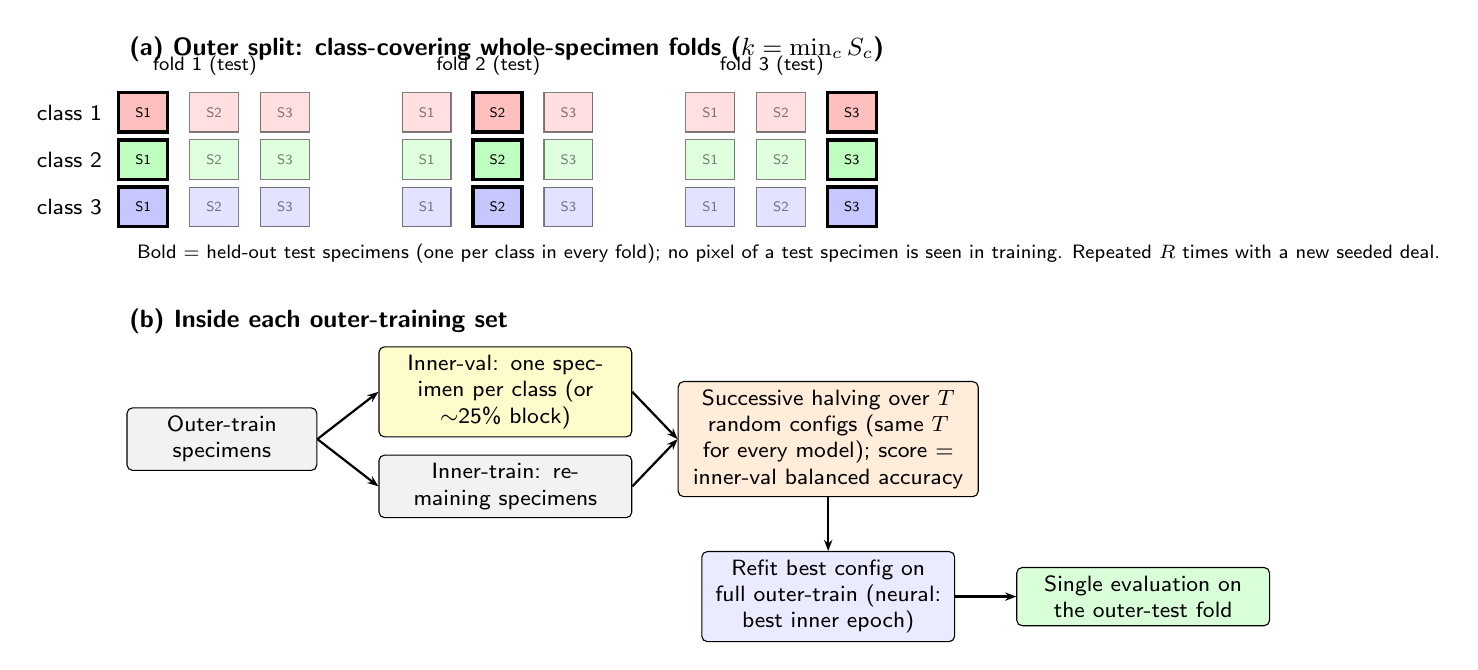
\begin{tikzpicture}[
  font=\sffamily\footnotesize,
  spec/.style={draw,minimum width=0.62cm,minimum height=0.5cm,inner sep=0pt,font=\sffamily\tiny},
  A/.style={spec,fill=red!25}, B/.style={spec,fill=green!25}, C/.style={spec,fill=blue!22},
  tst/.style={very thick,draw=black},
  box/.style={draw,rounded corners=2pt,align=center,fill=white,inner sep=3pt},
  arr/.style={-{Stealth[length=4pt]},thick}]

% (a) class covering folds: 3 classes x 3 specimens, k=3
\node[font=\sffamily\small\bfseries,anchor=west] at (0,2.35) {(a) Outer split: class-covering whole-specimen folds ($k=\min_c S_c$)};
\foreach \cls/\sty/\y in {1/A/1.55,2/B/0.95,3/C/0.35}{
  \node[anchor=east] at (-0.1,\y) {class \cls};
}
% fold 1..3 as three blocks side by side
\foreach \f [evaluate=\f as \x using {(\f-1)*3.6+0.3}] in {1,2,3}{
  \node[anchor=south west,font=\sffamily\scriptsize] at (\x,1.9) {fold \f\ (test)};
  \foreach \s in {1,2,3}{
    \pgfmathsetmacro{\sx}{\x+(\s-1)*0.9}
    \pgfmathtruncatemacro{\ist}{\s==\f}
    \foreach \sty/\y/\cls in {A/1.55/1,B/0.95/2,C/0.35/3}{
      \ifnum\ist=1
        \node[\sty,tst] at (\sx,\y) {S\s};
      \else
        \node[\sty,opacity=0.5] at (\sx,\y) {S\s};
      \fi
    }
  }
}
\node[font=\sffamily\scriptsize,anchor=west] at (0.1,-0.25)
  {Bold = held-out test specimens (one per class in every fold); no pixel of a test specimen is seen in training. Repeated $R$ times with a new seeded deal.};

% (b)
\node[font=\sffamily\small\bfseries,anchor=west] at (0,-1.1) {(b) Inside each outer-training set};
\node[box,fill=gray!10,text width=2.2cm] (otr) at (1.3,-2.6) {Outer-train specimens};
\node[box,fill=yellow!20,text width=3.0cm] (iv) at (4.9,-2.0) {Inner-val: one specimen per class (or $\sim$25\% block)};
\node[box,fill=gray!10,text width=3.0cm] (it) at (4.9,-3.2) {Inner-train: remaining specimens};
\draw[arr] (otr.east)--(iv.west); \draw[arr] (otr.east)--(it.west);
\node[box,fill=orange!15,text width=3.6cm] (sh) at (9.0,-2.6)
  {Successive halving over $T$ random configs (same $T$ for every model); score = inner-val balanced accuracy};
\draw[arr] (iv.east)--(sh.west); \draw[arr] (it.east)--(sh.west);
\node[box,fill=blue!8,text width=3.0cm] (refit) at (9.0,-4.6) {Refit best config on full outer-train (neural: best inner epoch)};
\draw[arr] (sh.south)--(refit.north);
\node[box,fill=green!15,text width=3.0cm] (ev) at (13.0,-4.6) {Single evaluation on the outer-test fold};
\draw[arr] (refit)--(ev);
\end{tikzpicture}
\end{document}
